\documentclass [11pt,twoside]{article}
\usepackage[utf8]{inputenc}
\usepackage[T1]{fontenc}

%Page margins, header and footer positions
\usepackage{geometry}
 \geometry{
 a4paper,
 total={210mm,297mm},
 left=25mm,
 right=25mm,
 top=30mm,
 bottom=25mm,
 headsep=7mm}

\interfootnotelinepenalty=10000

%To display filling dots in the TOC for all entries
\usepackage[titles]{tocloft}
\renewcommand{\cftsecleader}{\cftdotfill{\cftdotsep}}

%Define new header and footer style
\usepackage{fancyhdr}

\pagestyle{fancy}
\fancyhf{}
\lhead{\color{Gray}{\small{Travlendar+ project by YOUR NAMES}}}
\lfoot{\textcolor{Gray}{\small{Copyright © 2017, YOUR NAMES – All rights reserved}}}
\rfoot{\textcolor{Gray}{\thepage}}
\renewcommand{\headrulewidth}{0pt}

%PACKAGES
\usepackage{wasysym}
\usepackage{pifont}

\newcommand{\supported}{\ding{52}\xspace}
\newcommand{\unsupported}{\ding{55}\xspace}
\newcommand{\partsupported}{\textcolor{black!40}{\ding{52}}\xspace}
\newcommand{\lowsupported}{\textcolor{black!20}{\ding{52}}\xspace}
\newcommand{\unknowsupported}{\textbf{?}\xspace}

%Font: Times
\usepackage{times}
%Change monospaced font
\renewcommand{\ttdefault}{lmtt}

%tables
\usepackage{tabu}
\usepackage{tabularx}
\usepackage{ltablex}
\usepackage{longtable}
\usepackage{float} % To allow the use of H modifier in long tables

%landscape mode
\usepackage{pdflscape}
\usepackage{rotating}
\usepackage{caption}

%make landscape mode be sensitive to even and odd pages
%start
\def\myrotate{\ifodd\c@page\else-\fi 90}
\makeatletter
\global\let\orig@begin@landscape=\landscape%
\global\let\orig@end@landscape=\endlandscape%
\gdef\@true{1}
\gdef\@false{0}
\gdef\landscape{%
    \global\let\within@landscape=\@true%
    \orig@begin@landscape%
}%
\gdef\endlandscape{%
    \orig@end@landscape%
    \global\let\within@landscape=\@false%
}%
\@ifpackageloaded{pdflscape}{%
    \gdef\pdf@landscape@rotate{\PLS@Rotate}%
}{
    \gdef\pdf@landscape@rotate#1{}%
}
\let\latex@outputpage\@outputpage
\def\@outputpage{
    \ifx\within@landscape\@true%
        \if@twoside%
            \ifodd\c@page%
                \gdef\LS@rot{\setbox\@outputbox\vbox{%
                    \pdf@landscape@rotate{-90}%
                    \hbox{\rotatebox{90}{\hbox{\rotatebox{180}{\box\@outputbox}}}}}%
                }%
            \else%
                \gdef\LS@rot{\setbox\@outputbox\vbox{%
                    \pdf@landscape@rotate{+90}%
                    \hbox{\rotatebox{90}{\hbox{\rotatebox{0}{\box\@outputbox}}}}}%
                }%
            \fi%
        \else%
            \gdef\LS@rot{\setbox\@outputbox\vbox{%
                \pdf@landscape@rotate{+90}%
                \hbox{\rotatebox{90}{\hbox{\rotatebox{0}{\box\@outputbox}}}}}%
            }%
        \fi%
    \fi%
    \latex@outputpage%
}
\makeatother
%end

%graphics
\usepackage{graphicx}
\usepackage[dvipsnames, table]{xcolor}
%If you upload images from PC, you need to insert code for the path here (different for Windows and Unix OS)

%References
%\usepackage{xpatch}
%\usepackage[backend=biber, style=numeric, citestyle=numeric, sorting=none]{biblatex}
%\addbibresource{rasd.bib}

%Other
\usepackage{ifthen}
\usepackage{xspace}
\usepackage{enumitem}
\usepackage{amssymb}
\usepackage[pdftex, colorlinks]{hyperref}
\newcommand{\comment}[1]{{\color{Red}$\blacktriangleright$ Comment: #1 $\blacktriangleleft$}}


% Some utilities\ldots
\usepackage{soul}
\usepackage{tikz}

\usetikzlibrary{calc}
\usetikzlibrary{decorations.pathmorphing}


\makeatletter

\newcommand{\defhighlighter}[3][]{%
  \tikzset{every highlighter/.style={color=#2, fill opacity=#3, #1}}%
}

\defhighlighter{yellow}{.5}

\newcommand{\highlight@DoHighlight}{
  \fill [ decoration = {random steps, amplitude=1pt, segment length=15pt}
        , outer sep = -15pt, inner sep = 0pt, decorate
       , every highlighter, this highlighter ]
        ($(begin highlight)+(0,8pt)$) rectangle ($(end highlight)+(0,-3pt)$) ;
}

\newcommand{\highlight@BeginHighlight}{
  \coordinate (begin highlight) at (0,0) ;
}

\newcommand{\highlight@EndHighlight}{
  \coordinate (end highlight) at (0,0) ;
}

\newdimen\highlight@previous
\newdimen\highlight@current

\DeclareRobustCommand*\highlight[1][]{%
  \tikzset{this highlighter/.style={#1}}%
  \SOUL@setup
  %
  \def\SOUL@preamble{%
    \begin{tikzpicture}[overlay, remember picture]
      \highlight@BeginHighlight
      \highlight@EndHighlight
    \end{tikzpicture}%
  }%
  %
  \def\SOUL@postamble{%
    \begin{tikzpicture}[overlay, remember picture]
      \highlight@EndHighlight
      \highlight@DoHighlight
    \end{tikzpicture}%
  }%
  %
  \def\SOUL@everyhyphen{%
    \discretionary{%
      \SOUL@setkern\SOUL@hyphkern
      \SOUL@sethyphenchar
      \tikz[overlay, remember picture] \highlight@EndHighlight ;%
    }{%
    }{%
      \SOUL@setkern\SOUL@charkern
    }%
  }%
  %
  \def\SOUL@everyexhyphen##1{%
    \SOUL@setkern\SOUL@hyphkern
    \hbox{##1}%
    \discretionary{%
      \tikz[overlay, remember picture] \highlight@EndHighlight ;%
    }{%
    }{%
      \SOUL@setkern\SOUL@charkern
    }%
  }%
  %
  \def\SOUL@everysyllable{%
    \begin{tikzpicture}[overlay, remember picture]
      \path let \p0 = (begin highlight), \p1 = (0,0) in \pgfextra
        \global\highlight@previous=\y0
        \global\highlight@current =\y1
      \endpgfextra (0,0) ;
      \ifdim\highlight@current < \highlight@previous
        \highlight@DoHighlight
        \highlight@BeginHighlight
      \fi
    \end{tikzpicture}%
    \the\SOUL@syllable
    \tikz[overlay, remember picture] \highlight@EndHighlight ;%
  }%
  \SOUL@
}

\makeatother

% Common abbrev. are set as commands to ensure proper spacing after the dot
\RequirePackage{xspace}
\newcommand{\ie}{i.e.\@\xspace}
\newcommand{\aka}{a.k.a.\@\xspace}
\newcommand{\Ie}{I.e.\@\xspace}
\newcommand{\cf}{cf.\@\xspace}
\newcommand{\Cf}{Cf.\@\xspace}
\newcommand{\eg}{e.g.\@\xspace}
\newcommand{\Eg}{E.g.\@\xspace}
\newcommand{\etal}{et al.\@\xspace}
\newcommand{\etc}{etc.\@\xspace}
\newcommand{\wrt}{w.r.t.\@\xspace}
\newcommand{\Wrt}{W.r.t.\@\xspace}



\date{}


\begin{document}

\begin{titlepage}
	\begin{center}
		\line(1,0){400}\\	[0.6cm]
		\Huge{\bfseries{TRAVLENDAR+}}\\
		\line(1,0){400}\\
		[3cm]
		
\includegraphics[scale=0.3]{Images/polimi}\\
		[3cm]
		\textsc{\Huge Requirement Analysis and Specification Document}\\[1cm]
		\textsc{\huge 26/11/2017 - v1.1}\\
		[4cm]
		\textsc{\normalsize Matteo Colombo \hspace{0.4cm} Alessandro Perego \hspace{0.4cm} Andrea Troianiello }
	\end{center}
\end{titlepage}
	
%Deliverable specific info
\begin{table}[h!]
\begin{tabu} to \textwidth { X[0.3,r,p] X[0.7,l,p] }
\hline

\textbf{Deliverable:} & RASD\\
\textbf{Title:} & Requirement Analysis and Verification Document \\
\textbf{Authors:} & Matteo Colombo, Alessandro Perego, Andrea Troianiello \\
\textbf{Version:} & 1.1 \\ 
\textbf{Date:} & 26-November-2017 \\
\textbf{Download page:} & \href{https://github.com/MatteoColombo/ColomboPeregoTroianiello}{\color{Black}{GitHub - ColomboPeregoTroianiello repository}} \\
\hline
\end{tabu}
\end{table}

%------table of contents------%
\clearpage
\tableofcontents
\listoffigures
\listoftables


%------ CONTENT ------%

%------------------------------------------------------------------------------------------------------------------------------------------------
\clearpage
{\section{Introduction}}
\label{sect:introduction}
\subsection{Purpose}
This document is the baseline for project planning and for software evaluation of Travlendar+; it describes the system in terms of functional and nonfunctional requirements, analysing the needs of the customer in order to model the system.\\
Travlendar+ is a calendar-based application for people who have problems with scheduling working and personal appointments at various locations all across Milan. The application aims at simplifying the life of people by automatically computing travels and by organizing the daily schedules.

\subsection{Scope}
Travlendar+ is a calendar-based application whose purpose is to help people to easily schedule working or personal meetings around Milan.
Travlendar+ is intended to all people that need to organize their daily events and movements. The system-to-be will allow users to plan travels and meetings without worrying of being late or to miss lunch and, thanks to its high customizability, people will be able to save a lot of time. Alerts will be given when meetings are created at unreachable locations and travel means will be computed depending on day hours and weather.

\subsection{Definitions, Acronyms, Abbreviations}

\subsubsection{Definitions}
\begin{itemize}
\renewcommand{\labelitemi}{$-$}
\item
Schedule: set of meetings of the same day.
\item
Calendar: set of the schedules and from this you can select a specific schedule.
\item
Meeting: event in the schedule of the user that has a location and a start and end hour.
\item
Break: event that has a custom time range in which it can be schedule, with a minummum duration of 5 minutes.
\item
Lunch: it's a particular break with no customizable range time and minimum duration of 30 minutes.
\item
Travel pass: represents all type of passes (daily, weekly, monthly and yearly pass) for public transportations.
\item
Level: pollution level of a travel travel mean. 
\item
Event type: the type of a meeting (e.g. family, personal, work, etc). 
\end{itemize}


\subsubsection{Acronyms}
\begin{itemize}
\renewcommand{\labelitemi}{$-$}
\item
RASD: Requirement Analysis and Specification Document.
\item
IEEE: Institute of Electrical and Electronic Engineers.
\item
API: Application Programming Interface.
\end{itemize}

\subsubsection{Abbreviations}
\begin{itemize}
\renewcommand{\labelitemi}{$-$}
\item
$[$G.x$]$: the goal number x.
\item
$[$R.x.y$]$: the requirement number y of the goal x.
\item
$[$R.G.y$]$: the general requirement number y.
\item
$[$D.x$]$: the domain assumption number x.
\end{itemize}

\subsection{Revision History}
\begin{center}
\begin{longtable}{|p{2cm} | p{3cm}| p{8cm}|}
\hline \multicolumn{1}{|c|}{\textbf{Version}} & \multicolumn{1}{c|}{\textbf{Date}} & \multicolumn{1}{c|}{\textbf{Changes}} \\ \hline 
\endfirsthead
\hline
\endhead
\hline \multicolumn{3}{c}{{Continued on next page}} \\
\endfoot
\hline
\caption{Revision History}
\label{ref:revision}
\endlastfoot
v.1.0 & 29/10/2017 & Initial release \\
\hline 
v.1.1 & 26/11/2017 & Fix typos\\ 
\hline 
v.1.2 & 27/12/2017 & Improve sequence diagram and goals\\ 
\end{longtable}
\end{center}

\subsection{Reference Documents}
\begin{itemize}
\renewcommand{\labelitemi}{$-$}
\item
Specification Document: “Mandatory Project Assignments.pdf”.
\item
\href{http://ieeexplore.ieee.org/servlet/opac?punumber=6146377}{\color{Black}{IEEE Std 29148-2011 - ISO/IEC/IEEE International Standard - Systems and software engineering.}}
\item
Alloy Specification:\href{http://alloy.mit.edu/alloy/}{\color{Black}{"Software Abstractation", Daniel Jackson.}}
\item
Alloy:\href{http://tmancini.di.uniroma1.it/teaching/courses/2007-2008/mfis/materiale/progetti/Pagliaro\%20-\%20Alloy.relazione.pdf}{\color{Black}{"Alloy e l'Analyzer versione 4.0", "Alessandro Pagliaro"}}

\end{itemize}

\subsection{Document Structure}
This document is essentialy structured in four part:
\begin{itemize}
\item
Section 1: Introduction, this part gives a little description of the project and the definitions about terms and acronyms used in the document.
\item
Section 2: Overall Description, gives more information about the software product in particular its functions, constraints and assumptions.
\item
Section 3: Specific Requirements, describes the complete requirements of the project. You can see a list of possible scenarios, the use cases and the sequence diagram of the specific actions.
\item
Section 4: Alloy Description, this part is the representation of the structure of the project in Alloy language. You can see the entire code and the representation of one generated world.
\item
Section 5: This section contains the details about the efforts of each member of the group and the information about the software used in the writing of the document.
\end{itemize}

%------------------------------------------------------------------------------------------------------------------------------------------------
\clearpage
{\section{Overall Description}}
\label{sect:overview}
\subsection{Product Perspective}
Travlendar+ will be developed from scratch and it will be a mobile application that will require the user to have a smartphone with an internet connection and an integrated GPS system.

The application will allow the user to digitalize his schedule and will easily manage it.
When the user creates a new meeting, he is asked to provide the coordinates of the location, so that the application can compute the travel time to reach the meeting.
In this way the application makes sure that the user isn't ever late, because it permits to create a meeting only if it is reachable in time.

The application proposes only the best route for each travel that complies with the user preferences; this is achieved by using some external services like maps, public transportation and weather forecast providers.

During the journey, the application will assist the users by showing them the correct route or noticing them when they have to get off from public services.
Furthermore, through an external payment system, users are able to buy travel passes for their travels and visualize them directly in the application.

\subsubsection{Class Diagram}
The classes Event, Public Transportation, Travel Mean, Owned Vehicle and Shared Vehicle are abstract.\\
The classes that implement/extend Constraint, Level, Owned Mean, Shared Mean and Public Transportation are omitted for clarity.

\begin{figure}[h]
\centering
\includegraphics[scale=0.45]{images/classdiagram}
\caption{Class Diagram}
\label{fig:classdiagram}
\end{figure}


\begin{sidewaysfigure}
    \centering
	\includegraphics[scale=0.6]{images/classdiagram}
	\caption{Class Diagram}
	\label{fig:classdiagramrotate}
\end{sidewaysfigure}

\clearpage

\subsection{Product Functions}

\newcounter{gcount}
\newcounter{rcount}
\begin{list}
{\bfseries{}[G.\arabic{gcount}]~}
{
\usecounter{gcount}
}
\item Visitors can create an account.
\begin{list}
	{\bfseries{}[R.\arabic{gcount}.\arabic{rcount}]~}
	{
	\usecounter{rcount}
	}
\item An account requires an username.
\item An account requires an email address.
\item An account requires a password.
\item The email address must be unique.
\end{list}
\item Users can create new meetings.
\begin{list}
	{\bfseries{}[R.\arabic{gcount}.\arabic{rcount}]~}
	{
	\usecounter{rcount}
	}
	\item The user must be logged in the application.
\item A meeting requires a location, which is either coordinates or an address.
\item A meeting requires a starting and ending hour.
\item A meeting requires a name.
\item A meeting requires a type.
\item A meeting may have a description.
\end{list}
\item Warnings are shown in case a new meeting is unreachable or causes conflicts.
\begin{list}
	{\bfseries{}[R.\arabic{gcount}.\arabic{rcount}]~}
	{
	\usecounter{rcount}
	}
\item A warning should be given at the creation of a meeting if it is unreachable or if it is causes conflicts.
\item A warning should be given in case of exceptional events that make one or more meetings unreachable.
\item A warning forbids the user to force the creation of a meeting.
\end{list}
\item Travel means are suggested depending on different constraints.
\begin{list}
	{\bfseries{}[R.\arabic{gcount}.\arabic{rcount}]~}
	{
	\usecounter{rcount}
	}
\item Different travel means should be suggested depending on the weather conditions.
\item Different type of meetings should be reached with different/specific travel means.
\item Different travel means should be suggested depending on the hour of the day.
\item Travel means can have constraints on the length of their journey section.
\end{list}
\item Users can set their preferences and select between different options.
\begin{list}
	{\bfseries{}[R.\arabic{gcount}.\arabic{rcount}]~}
	{
	\usecounter{rcount}
	}
\item The application must support different travel means and transportation systems.
\item Users can select constraints on travel means.
\item The application must show results consistent with the users preferences.
\item Users should be able to specify the travel passes they own.
\item Users must specify their home address.
	\item Users can disable travel means.
	\item Users can enable the option to minimize air pollution.
    \end{list}
\item Lunch breaks are automatically scheduled by the application.
\begin{list}
	{\bfseries{}[R.\arabic{gcount}.\arabic{rcount}]~}
	{
	\usecounter{rcount}
	}
\item The minimum length of a lunch break is 30 minutes.
\item The lunch break must be scheduled between 11.30 am and 2.30pm.
\end{list}
\item Users can add custom breaks that are automatically scheduled.
\begin{list}
	{\bfseries{}[R.\arabic{gcount}.\arabic{rcount}]~}
	{
	\usecounter{rcount}
	}
\item The minimum length of a lunch break is 5 minutes.
\item Users can set as many breaks as they want.
\item Users can select the time slot in which they want their break to be scheduled.
\end{list}
\item Users are assisted during their journey.
\begin{list}
	{\bfseries{}[R.\arabic{gcount}.\arabic{rcount}]~}
	{
	\usecounter{rcount}
	}
\item The application should notify the user when he has to get off from a transportation system.
\item The applications should give directions to the users when they are driving, cycling or walking.
\item Users can buy travel passes through the application.
\item The application must locate the nearest vehicle of the selected sharing system.
\end{list}


\end{list}

\subsection{User Characteristics}

\subsubsection{Principal Actors}

\renewcommand{\labelitemi}{$-$}
\begin{itemize}
\item
Visitor: a person using Travlendar+ without being signed-up. He is able to proceed with registration or log-in.
\item
User: a person has successful login and can use the app services. He can manage his preferences and his appointments.
\end{itemize}

\subsubsection{Secondary Actors}
There are some secondary actors such as third party service providers, that are needed by the system to retrieve information, used to perform payments or to compute the travel options. 

\subsection{Assumptions and Dependencies}
\subsubsection{Domain Assumptions}
\newcounter{tcount}
\begin{list}
{\bfseries{}[D.\arabic{tcount}]~}
{
\usecounter{tcount}
}
\item
The time slot in which lunch can be scheduled is between 11.30am and 2.30pm.
\item
The minimum duration for a lunch break is 30 minutes.
\item
Breaks work in the same way of lunch, but their time slot can be customized by the user.
\item
The minimum duration of a break is 5 minutes.
\item
A meeting is always associated to a position.
\item
When a user adds a new meeting, if the application detects that it causes one of the following errors, it forces the user to edit the information of the meeting. Errors:

\begin{enumerate}
\item
The meeting overlaps with another.
\item
The meeting is unreachable.
\item
The meeting makes another unreachable.
\item
The meeting doesn't leave enough time for lunch.
\end{enumerate}


\item
In case of a long travel that overlaps with the lunch break and doesn’t give enough time to the lunch in (but there is enough time after the lunch slot), it may be splitted in two parts, separated by the break. The same applies for afternoon/morning breaks.
\item
The application gives higher priority at moving breaks at the beginning of their dedicated time slot.
\item
The application tries to maximize the duration of the breaks.
\item
The daily schedule starts at the user's home and ends at the last meeting of the day.
\item
An event starts and ends always in the same calendar day.
\item
GPS has a precision of 3m.
\item
When creating a meeting, the position typed by the user is used as meeting location to compute the travel time; while during the navigation or when the user is attending a meeting, the application retrieves his real location through GPS and updates travels times with it.
\item
The user can select a preferred travel mean for each type of meeting, so that depending on the type, the application prefers different travel means. For example, if for family meetings “car” is the preferred travel mean, if it is available, it would be the suggested mean, even if better options exist.
\item
Travel means can be subjected to different type of constraints, some chosen by the user other by the application.
\item
Travel means are classified by their footprint level.Travel passes can be of different types:
\begin{enumerate}
\item
Daily pass.
\item
Weekly pass.
\item
Monthly pass.
\item
Yearly pass.
\end{enumerate}

\item
A travel pass can be used only for one transportation mean. For example, a bus ticket can't be used for a tram journey.
\item
Cars and Bike are of two types: shared and owned.
\item
At least one vehicle of a sharing system can always be found within a 10 minute walk.
\item
Each vehicle of a sharing system can be located through GPS.
\item
During a single journey, many different travel means can be used.
\item
Public transports are always on time.
\item
Strikes or public transportation fault are communicated on the website of the service provider. 
\item
The system suggests to the user the best journey that complies with the users preferences.
\item
Meetings can be of three types: family, work and personal.
\item
The server is used for account related purposes and as backup.
\item
When a new meeting is created, the application synchronizes the schedule with the server.
\item
If when a new meeting is created the connection to the server isn't available, the meeting is created anyhow and the synchronization will be done when the connection returns.
\item
If a conflict is generated when the user tries to change the time slot dedicated to a break, a warning is shown and the change fordbidden.
\end{list}

%------------------------------------------------------------------------------------------------------------------------------------------------
\clearpage
{\section{Specific Requirements}}
\label{sect:requirements}
All the decisions in the DD have been taken following functional and nonfunctional requirements written in the RASD. In this chapter, each requirement is mapped to specific component.
\\
\begin{itemize}

\item
\textbf{LoginManager:}
\begin{itemize}
\item
$[$R.1.1$]$ An account requires an username.
\item
$[$R.1.2$]$ An account requires an email address.
\item 
$[$R.1.3$]$ An account requires a password.
\item
$[$R.1.4$]$ The email address must be unique.
\item
$[$R.2.1$]$ The user must be logged in the application.
\end{itemize}

\item
\textbf{EventManager:}
\begin{itemize}
\item
$[$R.2.2$]$ A meeting requires a location, which is either coordinates or an address.
\item
$[$R.2.3$]$ A meeting requires a starting and ending hour.
\item
$[$R.2.4$]$ A meeting requires a name.
\item
$[$R.2.5$]$ A meeting requires a type.
\item
$[$R.2.6$]$ A meeting may have a description.
\item
$[$R.3.1$]$ A warning should be given at the creation of a meeting if it is unreachable or if
it is causes conflicts.
\item
$[$R.3.2$]$ A warning should be given in case of exceptional events that make one or more
meetings unreachable.
\item
$[$R.3.3$]$ A warning forbids the user to force the creation of a meeting.
\item
$[$R.6.1$]$ The minimum length of a lunch break is 30 minutes.
\item
$[$R.6.2$]$ The lunch break must be scheduled between 11.30 am and 2.30pm.
\item
$[$R.7.1$]$ The minimum length of a lunch break is 5 minutes.
\end{itemize}

\item
\textbf{Configurator:}
\begin{itemize}
\item
$[$R.4.2$]$ Different type of meetings should be reached with different/specific travel means.
\item
$[$R.4.3$]$ Different travel means should be suggested depending on the hour of the day.
\item
$[$R.4.4$]$ Travel means can have constraints on the length of their journey section.
\item
$[$R.5.1$]$ The application must support different travel means and transportation systems.
\item
$[$R.5.2$]$ Users can select constraints on travel means.
\item
$[$R.5.3$]$ The application must show results consistent with the users preferences.
\item
$[$R.5.4$]$ Users should be able to specify the travel passes they own.
\item
$[$R.5.5$]$ Users must specify their home address.
\item
$[$R.5.6$]$ Users can disable travel means.
\item
$[$R.5.7$]$ Users can enable the option to minimize air pollution.
\item
$[$R.7.2$]$ Users can set as many breaks as they want.
\item
$[$R.7.3$]$ Users can select the time slot in which they want their break to be scheduled.
\end{itemize}

\item
\textbf{JourneyManager:}
\begin{itemize}
\item
$[$R.4.1$]$ Different travel means should be suggested depending on the weather conditions.
\item
$[$R.4.3$]$ Different travel means should be suggested depending on the hour of the day.
\item
$[$R.8.1$]$ The application should notify the user when he has to get off from a transportation system.
\item
$[$R.8.2$]$ The applications should give directions to the users when they are driving, cycling or walking.
\end{itemize}

\item
\textbf{PaymentHandler:}
\begin{itemize}
\item
$[$R.8.3$]$ Users can buy travel passes through the application.
\end{itemize}

\item
\textbf{SharedController:}
\begin{itemize}
\item
$[$R.8.4$]$ The application must locate the nearest vehicle of the selected sharing system.
\end{itemize}
\end{itemize}

%------------------------------------------------------------------------------------------------------------------------------------------------
\clearpage
{\section{Formal Analysis Using Alloy}}
\label{sect:alloy}
\subsection{Alloy}
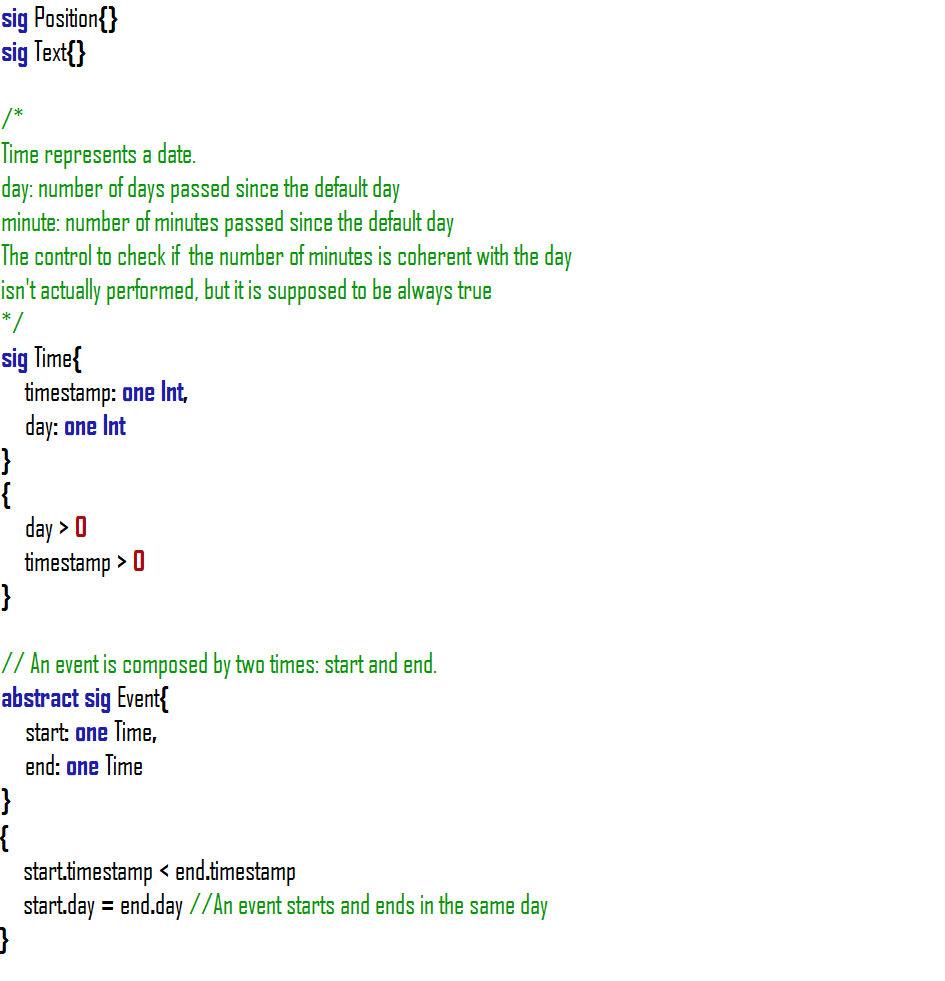
\includegraphics[scale=1]{Images/alloy1}
\clearpage
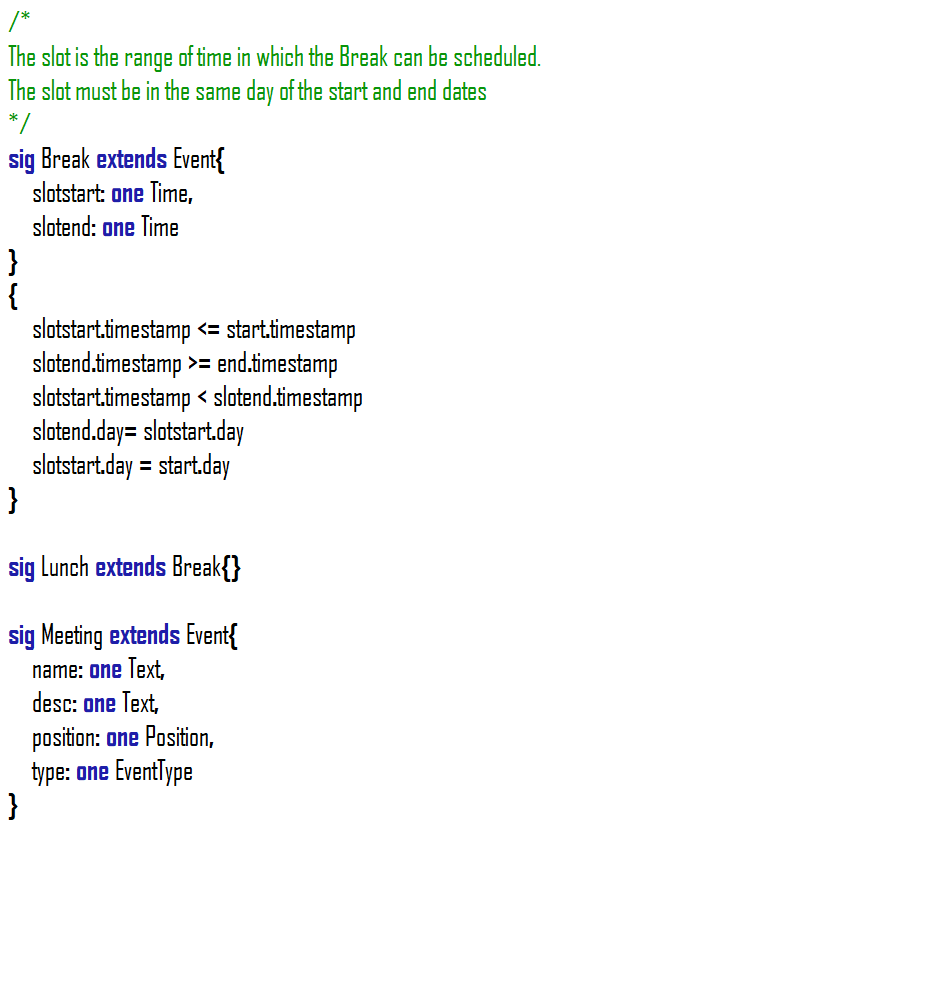
\includegraphics[scale=1]{Images/alloy2}
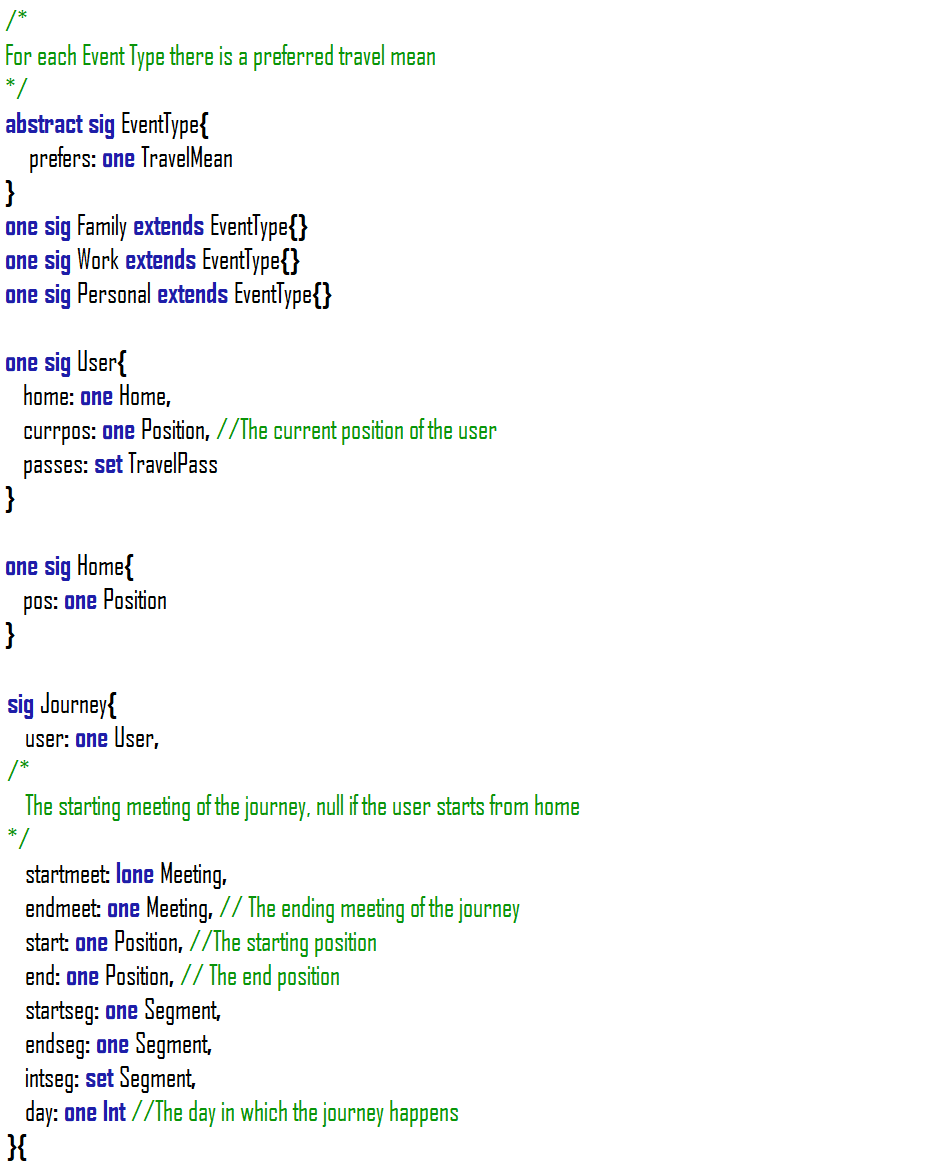
\includegraphics[scale=1]{Images/alloy3}
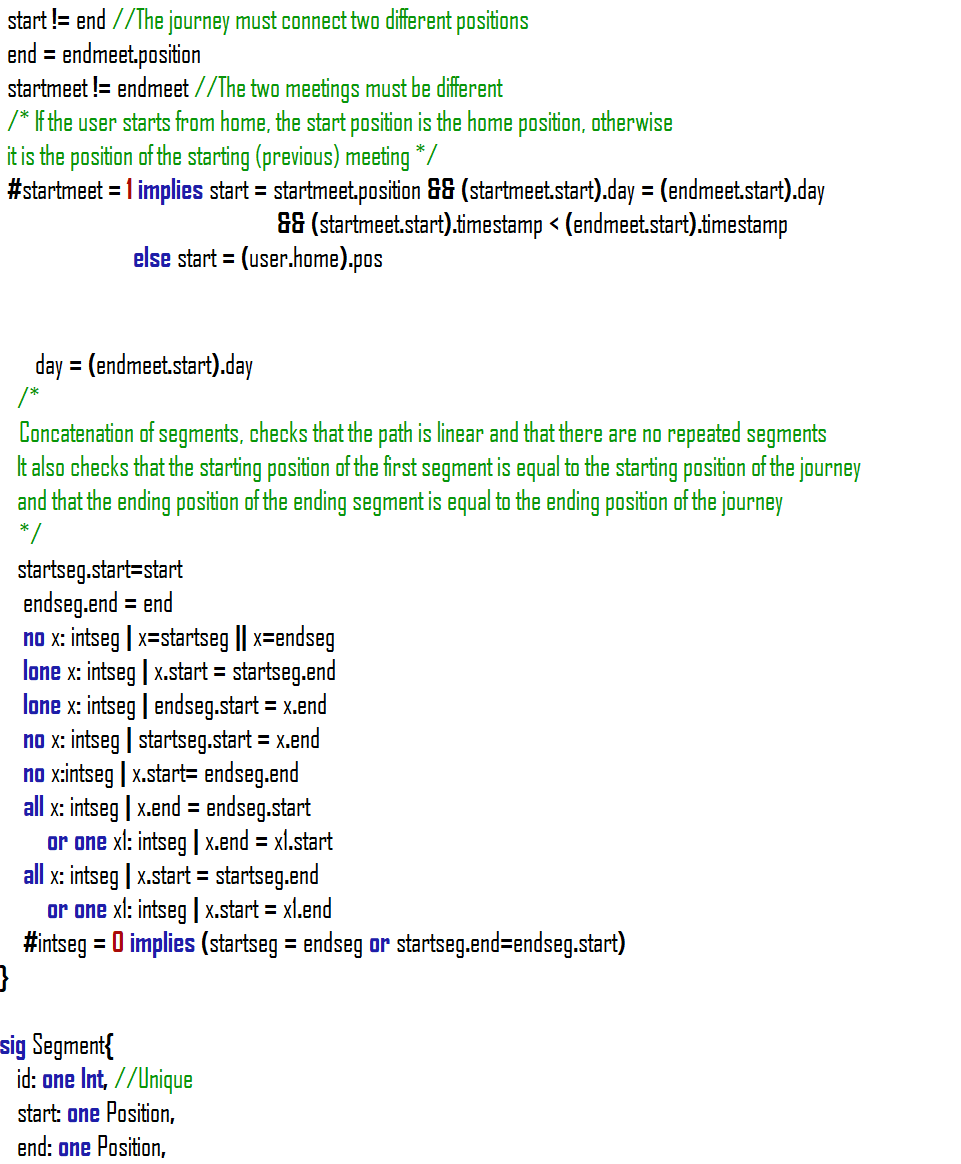
\includegraphics[scale=1]{Images/alloy4}
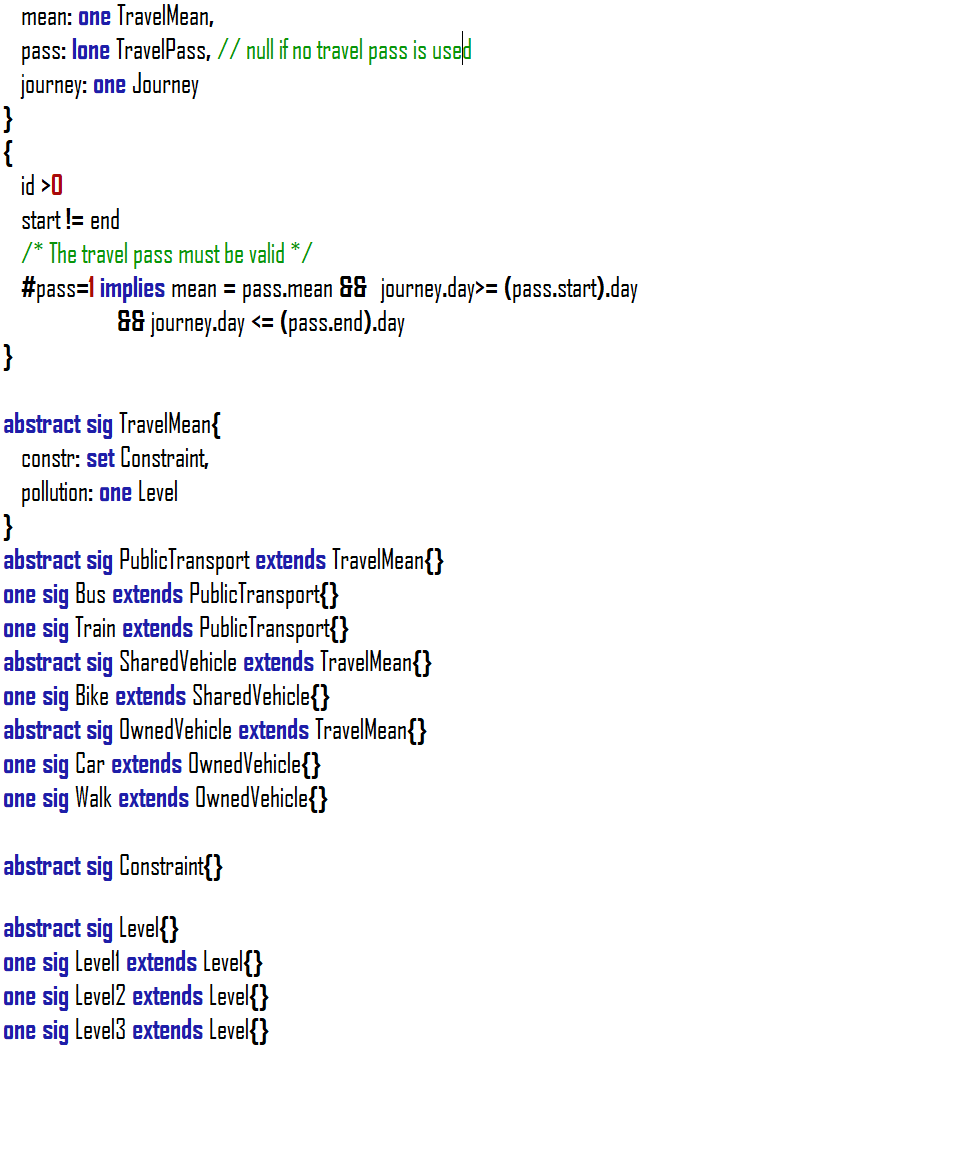
\includegraphics[scale=1]{Images/alloy5}
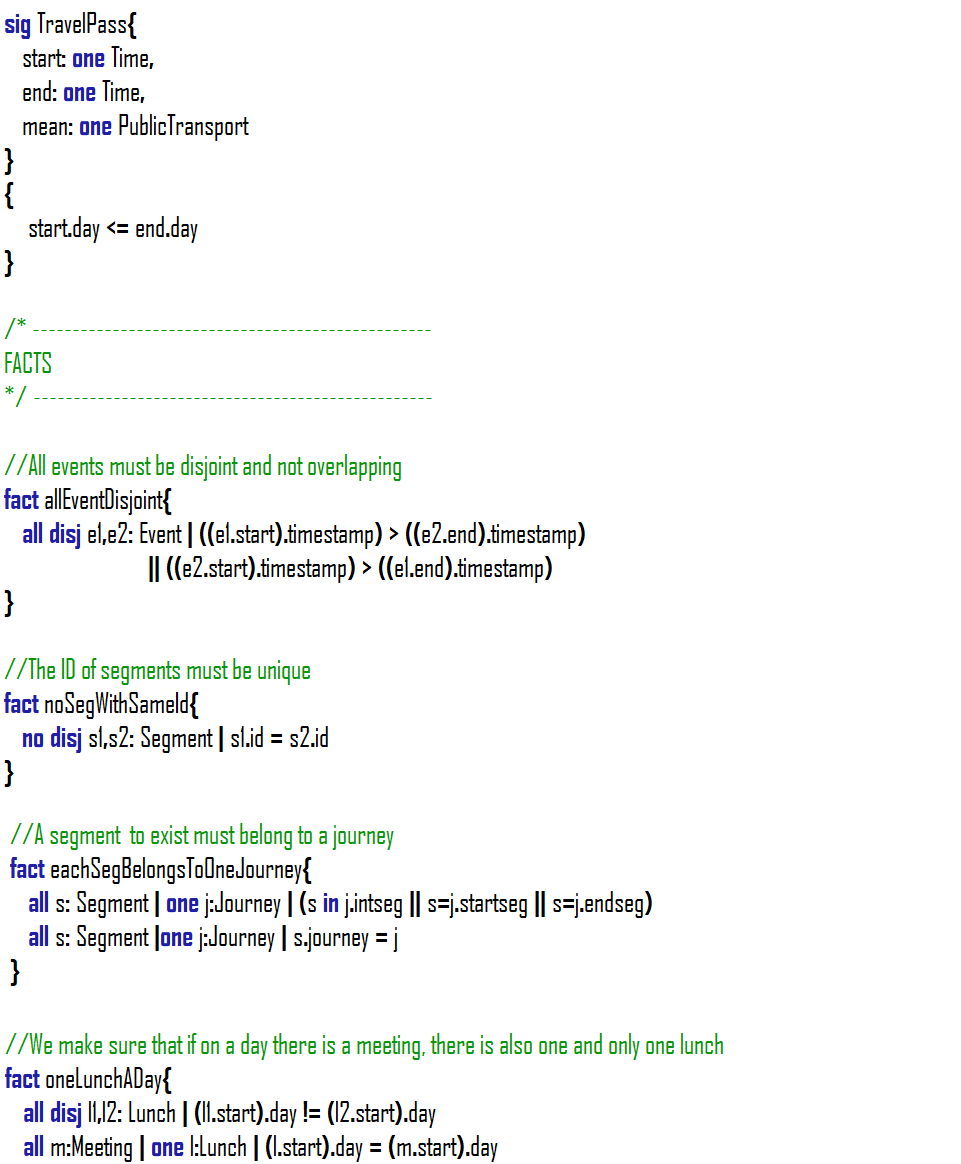
\includegraphics[scale=1]{Images/alloy6}
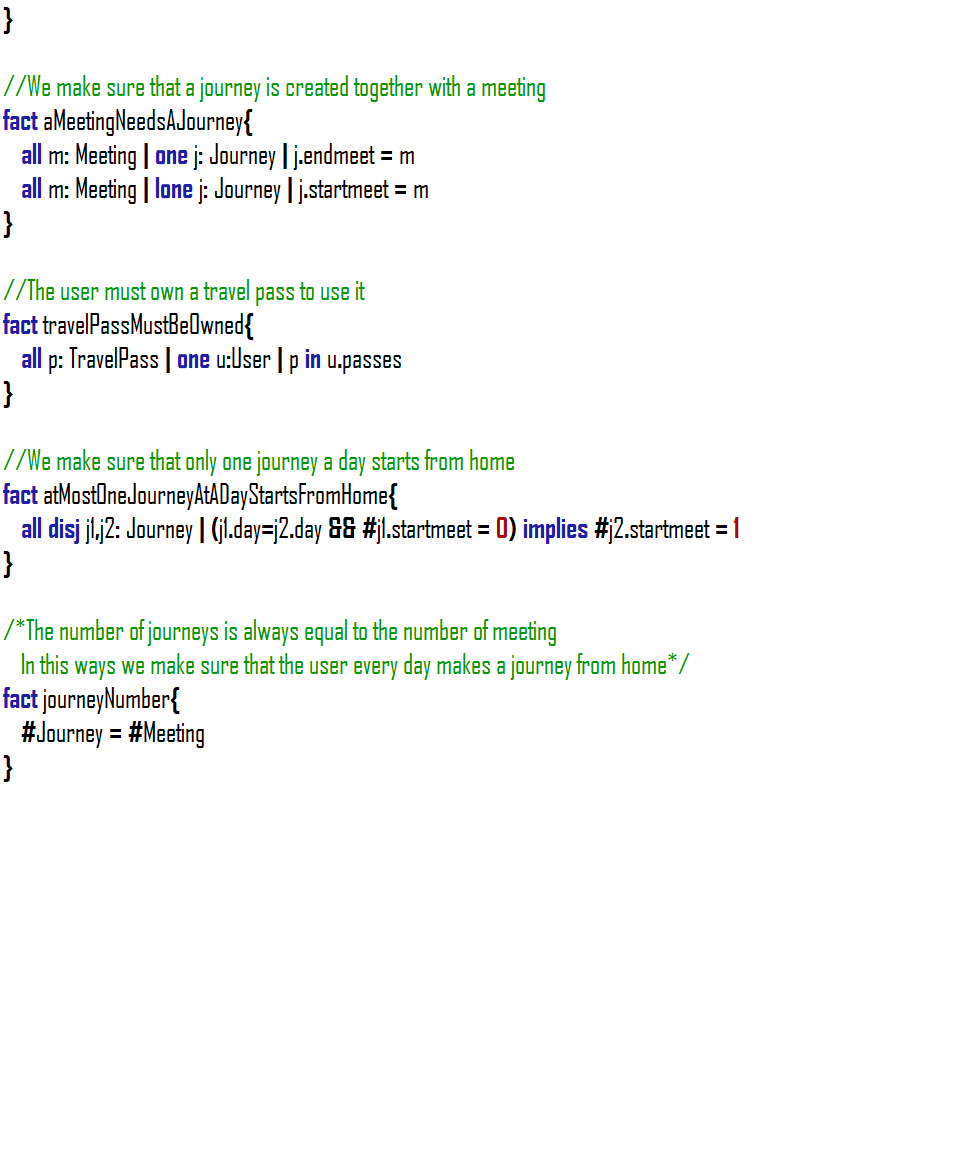
\includegraphics[scale=1]{Images/alloy7}
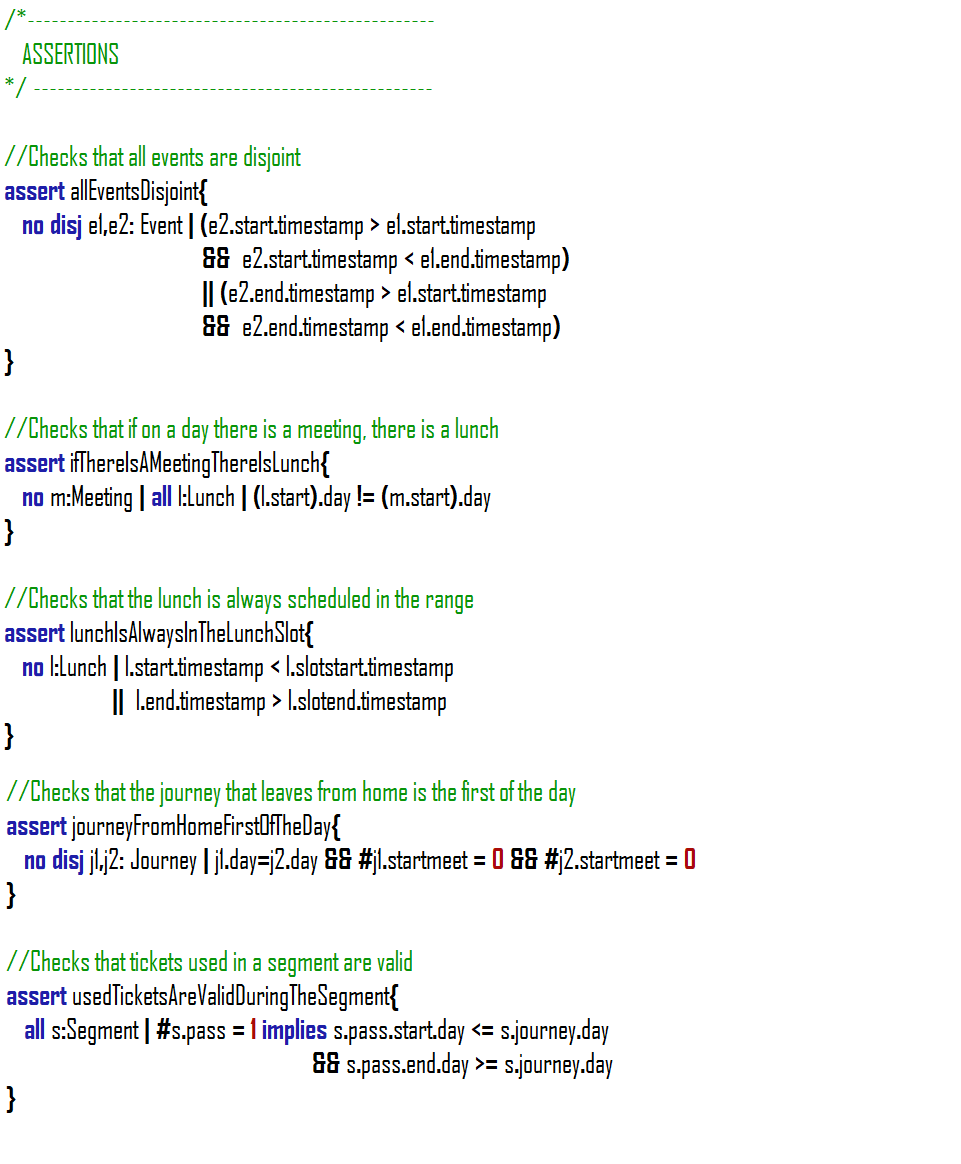
\includegraphics[scale=1]{Images/alloy8}
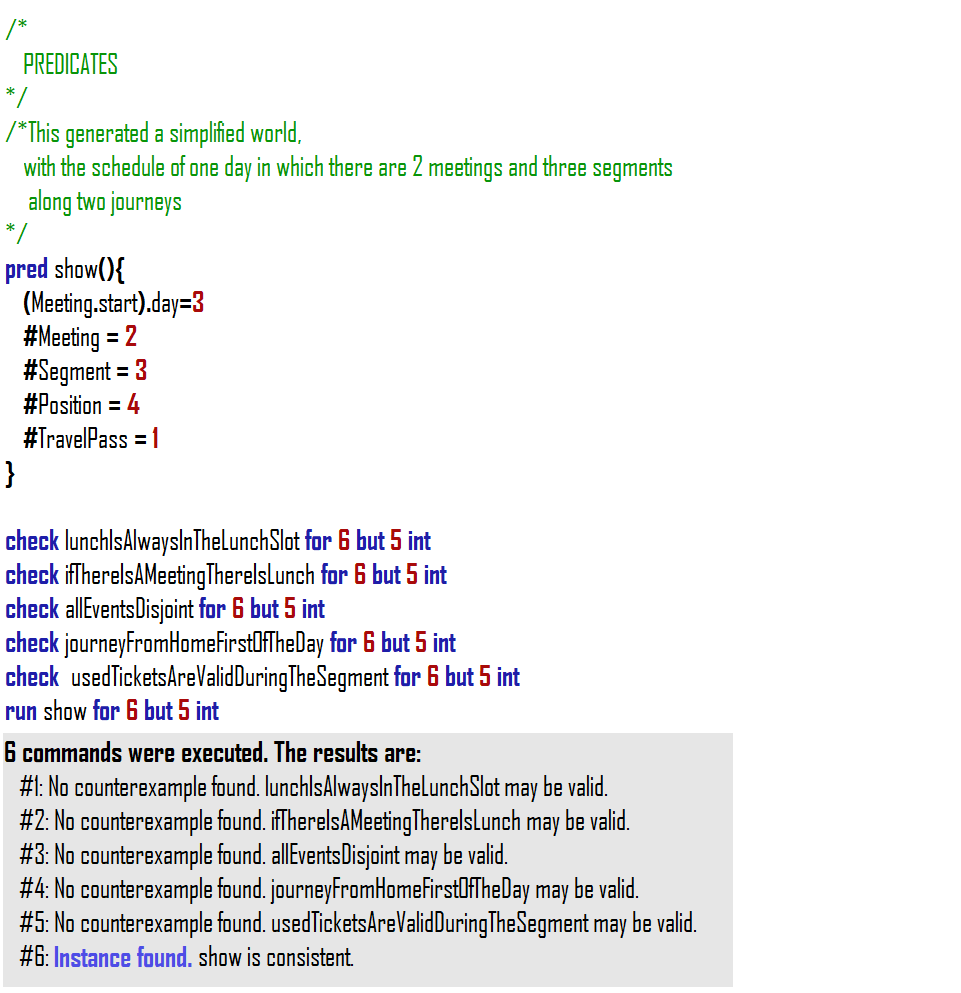
\includegraphics[scale=1]{Images/alloy9}

\clearpage
\subsection{Generated World}

\begin{figure}[htb]
\centering
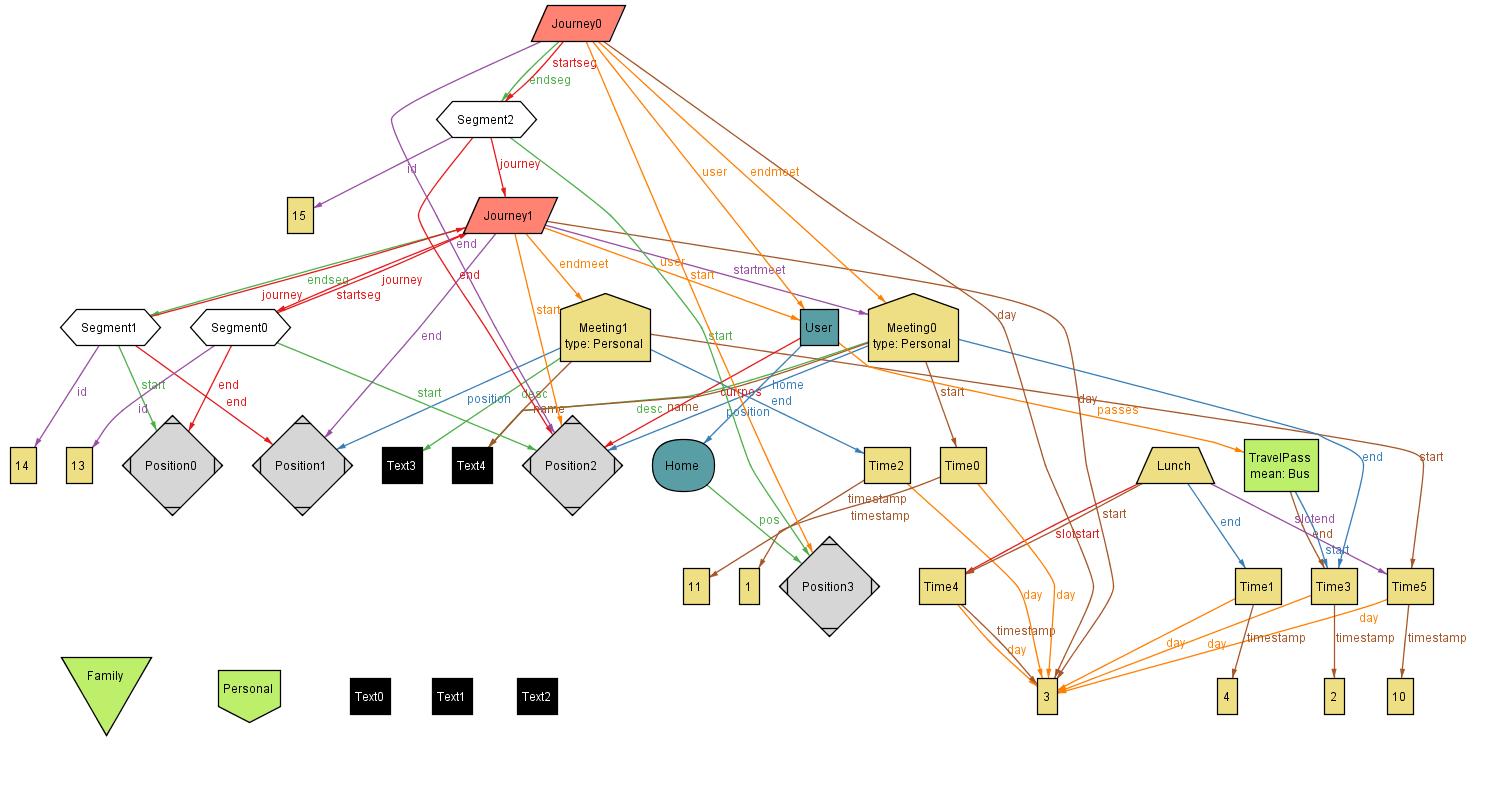
\includegraphics[scale=0.55]{Images/world2}
\caption{Generated World Magic Layout}
\label{fig:generatedworldmagic}
\end{figure}

\begin{sidewaysfigure}
\centering
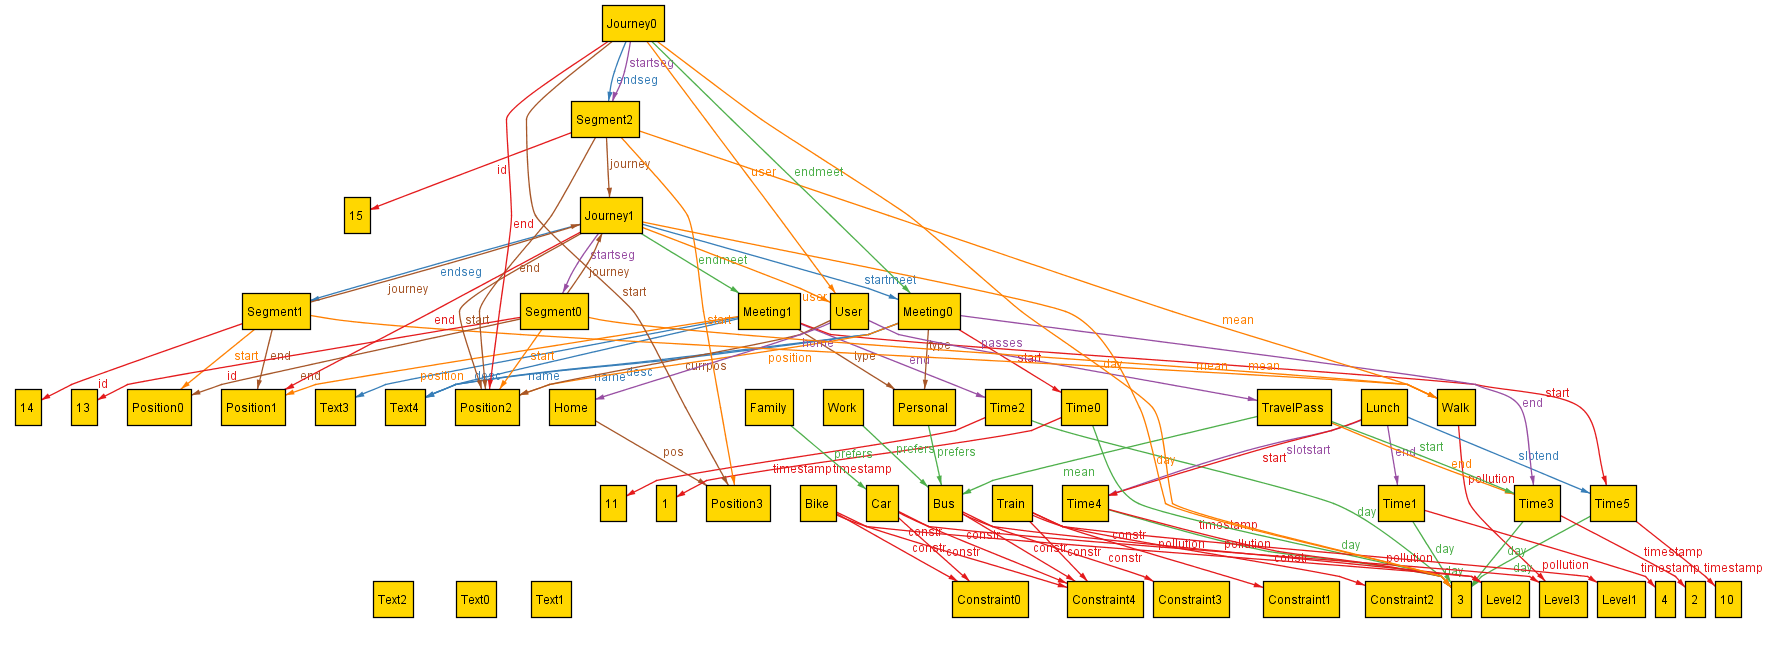
\includegraphics[scale=0.65]{Images/world1}
\caption{Generated World}
\label{fig:generatedworld}
\end{sidewaysfigure}

%------------------------------------------------------------------------------------------------------------------------------------------------
\clearpage
{\section{Effort Spent}}
\label{sect:effort}
\subsection{Time Spent}

\begin{center}
\begin{longtable}{|p{8cm} | p{5cm}|}
\hline \multicolumn{1}{|c|}{\textbf{Member}} & \multicolumn{1}{c|}{\textbf{Hours}} \\ \hline 
\endfirsthead
\hline
\endhead
\hline \multicolumn{2}{c}{{Continued on next page}} \\
\endfoot
\hline
\caption{Time Spent}
\label{ref:timespent}
\endlastfoot
Colombo Matteo & 45 \\
\hline 
Perego Alessandro & 45 \\ 
\hline
Troianiello Andrea & 45 \\
\end{longtable}
\end{center}
The commits on GitHub are not completely representative of the work done, a good part of it has been done in group.

\subsection{Used Tools}

\begin{enumerate}
\item
TexMaker for the editing of the LaTeX document.
\item
Star UML for the creation of UML diagrams (Class,Use Cases and Sequence diagrams).
\item
Balsamiq for the creation of the Mockup.
\item
Alloy Analyzer 4.2 for alloy analysis.
\end{enumerate}


%------------------------------------------------------------------------------------------------------------------------------------------------
\clearpage
\addcontentsline{toc}{section}{References}
\bibliographystyle{plain}
\bibliography{RASD}
%------------------------------------------------------------------------------------------------------------------------------------------------



\end{document}